\documentclass[10pt,a4paper]{article}
\usepackage[utf8]{inputenc}
\usepackage[german]{babel}
\usepackage{amsmath}
\usepackage{amsfonts}
\usepackage{amssymb}
\usepackage{siunitx}
\usepackage{multirow}
\usepackage[left=2cm,right=2cm,top=2cm,bottom=2cm]{geometry}
\usepackage{wrapfig}
\usepackage{graphicx}
\usepackage{caption}
\usepackage[colorlinks]{hyperref}


\author{Christian Bespin \and Christopher Deutsch}
\title{Übungsblatt 3: Numerische Methoden der Physik}
\begin{document}
\maketitle

\setcounter{section}{1}

\section{Treibhauseffekt}

\subsection{Physikalischer Hintergrund}

Wir verwenden zur Erklärung des Treibhauseffektes ein einfaches Modell grauer und schwarzer Körper. Die Erde entspricht dabei einem schwarzen Körper, das heißt Emissionsgrad ist gleich $1$, mit der Temperatur $T_E$. Die Sonne wird als grauer Körper mit konstanter Emissivität $\epsilon_S$ und ebenfalls konstanter Temperatur $T_S$. Im Gegensatz zum schwarzen Körper, absorbiert der graue Körper nicht die gesamte auf ihn treffende Strahlung und emittiert entsprechend auch nicht die maximal mögliche Schwarzkörperstrahlung. Es gilt daher, dass $\epsilon_{S}<1$. Im verwendeten Modell hat die Atmosphäre die Emissivität $\epsilon$ und die Temperatur $\tau$. Die Atmosphäre absorbiert den Anteil $\epsilon(T_S)$ der von der Sonne emittierte Srahlung, lässt entsprechend den Anteil $1-\epsilon(T_S)$ dieser Strahlung zur Erde durch und emittiert selber eine Strahlung mit Anteil $\epsilon(\tau)$. Letzteres, sowie die zur Berechnung benötigten Formeln sind unter $(1)$-$(3)$ auf dem Aufgabenzettel zu finden.\\
Die Temperaturen der Körper ändern sich je nach abgestrahlter und emittierter Strahlung, bis sich irgendwann ein Strahlungsgleichgewicht einstellt. In diesem strahlen alle Körper genau so viel ab, wie sie absorbieren und alle Temperaturen sind gleich der Endtemperatur.
\begin{figure}[htbp]
\centering
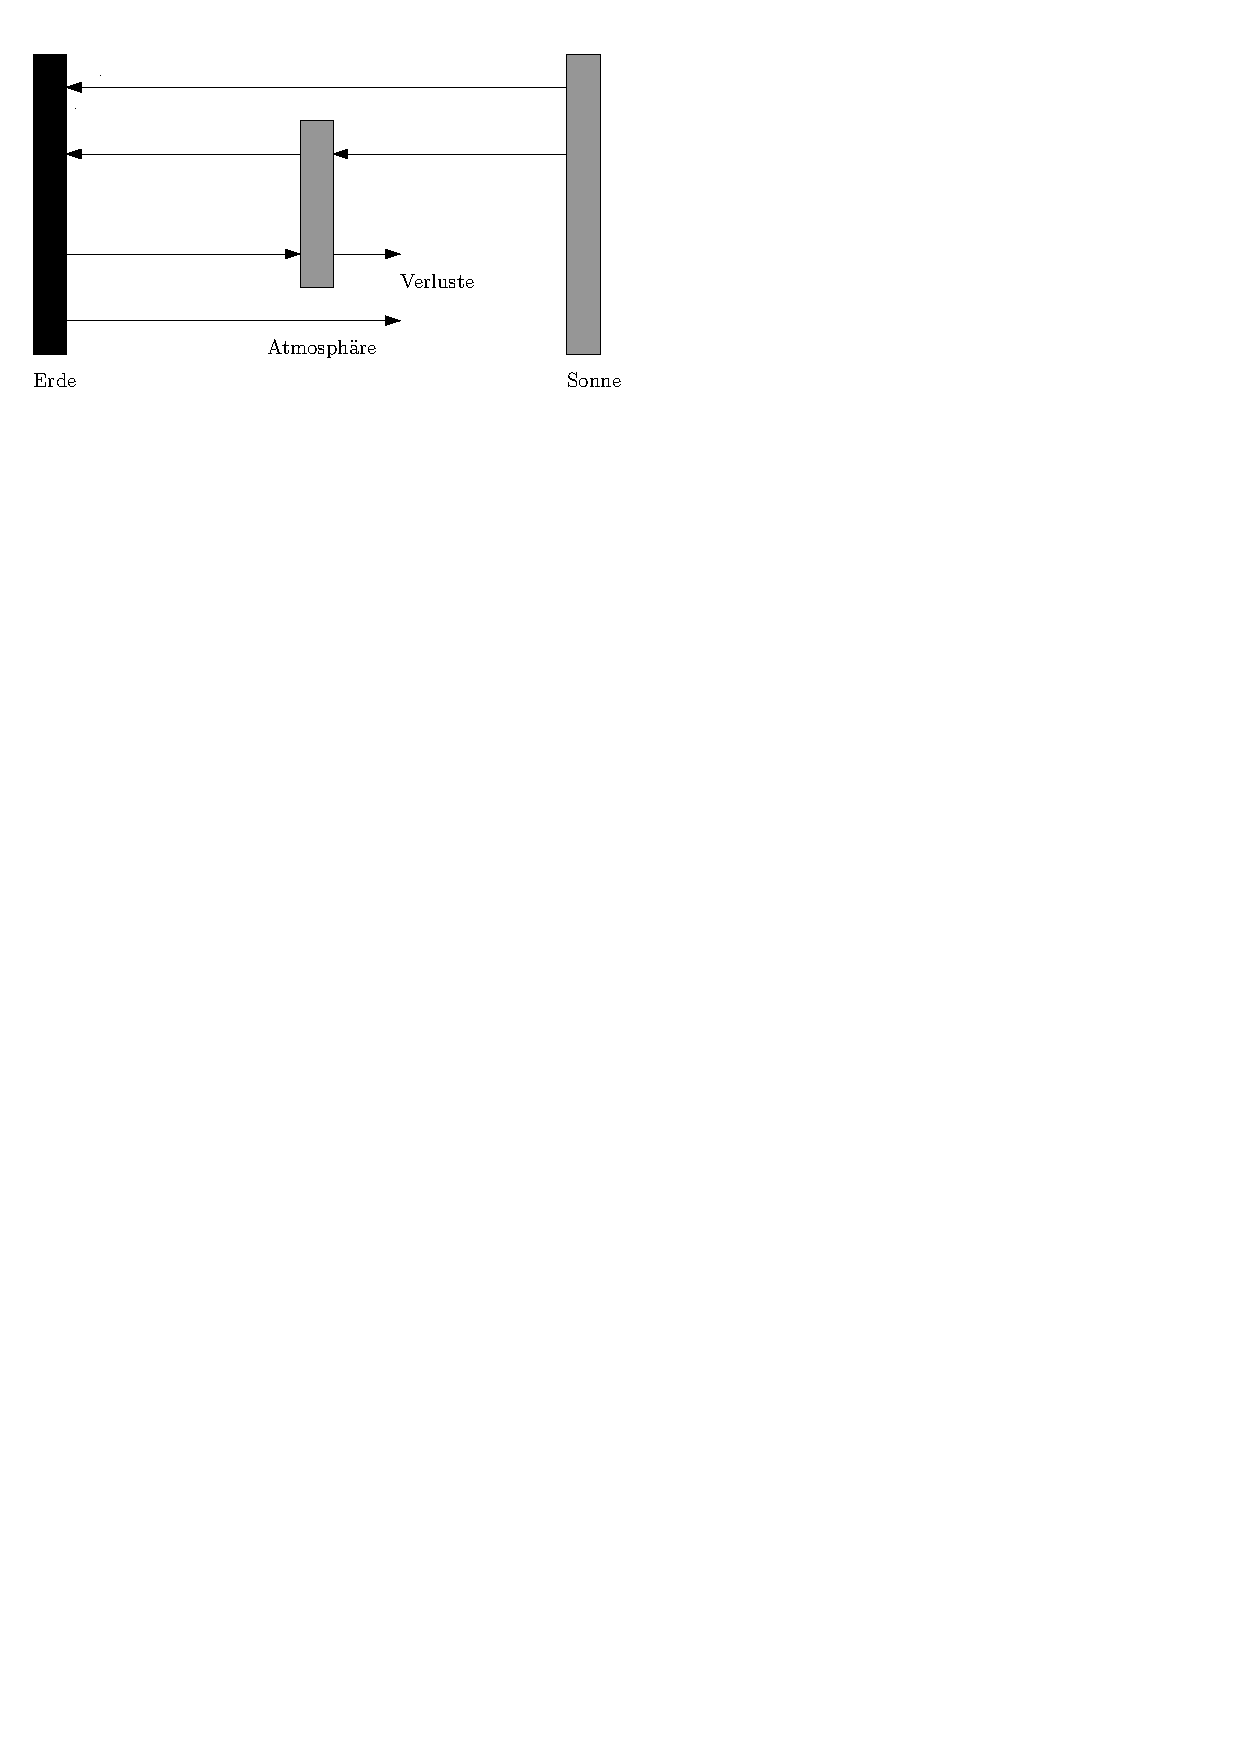
\includegraphics[height=5cm]{./figures/strahlungsgleichgewicht.pdf}
\caption{Strahlungsgleichgewicht}
\label{fig:strahlungsgleichgewicht}
\end{figure}
Im Strahlungsgleichgewicht gilt für unsere Modellannahme nach $(4)$ vom Aufgabenblatt:
\begin{align}
\left[2-\epsilon(T_E)\right]T_E^4=\epsilon_S\left[2-\epsilon(T_S)\right]T_S^4
\label{eqn:gleichgewicht}
\end{align}
Um $T_E$ zu bestimmen, muss man \ref{eqn:gleichgewicht} umstellen, so dass sich ein Nullstellenproblem ergibt:
\begin{align}
\left[2-\epsilon(T_E)\right]T_E^4-\epsilon_S\left[2-\epsilon(T_S)\right]T_S^4=0
\label{eqn:nullstellenform}
\end{align}
Der hintere Term hängt nicht von $T_E$ ab und kann mit geeigneten Verfahren (s.u.) zu einer konstanten Zahl bestimmt werden.
$\nu_{max}=T\cdot 5,8789254\num{1E10}\si{\per\second}\si{\per\kelvin}$ \footnote{http://physics.nist.gov/constants, Wien frequency displacement law constant}

\subsection{Mathematischer Hintergrund}

\subsection{Implementierung}

\subsubsection{Struktur des Programmes}

\subsubsection{Abbruchbedingungen}

\subsubsection{Genaugkeit}

\subsection{Physikalische Ergebnisse}
\label{ssec:physikalischeergebnisse}

\begin{thebibliography}{9}

\bibitem{abramowitzstegun}
Abramowitz, M. \& Stegun, I. A.
\emph{Handbook of Mathematical Functions},
Dover Books (1965)

\bibitem{healdmarion}
Heald, M. \& Marion, J.
\emph{Classical Electromagnetic Radiation},
Brooks Cole (1994)

\bibitem{kazimierczuk}
Kazimierczuk, M.
\emph{High-Frequency Magnetic Components},
Wiley (2009)

\bibitem{crchandbook}
David R. Lide (ed),
\emph{CRC Handbook of Chemistry and Physics},
84th Edition. CRC Press. Boca Raton, Florida, 2003;
Section 12, Properties of Solids; Electrical Resistivity of Pure Metals;
Section 4, The Elements: Magnetic Susceptibility

\end{thebibliography}

\end{document}
